\section{Discrete Optimization}

\begin{frame}

\slidesonly{
\begin{block}{Supervised \& unsupervised learning $\rightarrow$ evaluation of cost function $E$}
Find the arguments that optimize $E$.
\begin{itemize}
 \item real-valued arguments: gradient based techniques (e.g. ICA unmixing matrices)
 \item discrete arguments: ??? (e.g. for cluster assignment)
\end{itemize}
\end{block}
}
\notesonly{
So far we've been concerned with optimization problems with real valued arguments. The free parameters form a continuous space. The direction of the principle components in PCA and the unmixing matrix we are trying to find in ICA are real-valued arguments to their respective problems.
Gradient-based solutions are well suited for real-valued arguments as we tune the weights to minimize to optimize the cost function.

But what if the problem we are trying to optimize operate on discrete arguments. This could be the case if we were tackling a problem such as K-Means clustering. K-Means clustering involves finding arguments with which to assign an observation to one of multiple clusters. The cost function that measures the quality of the assignments is continuous but the arguments we optimize over, which effectively assign each observation to one cluster instead of another cluster, are discrete variables. Below is an example of such an assignment:


}

\only<1>{

\begin{figure}[ht]
  \centering
  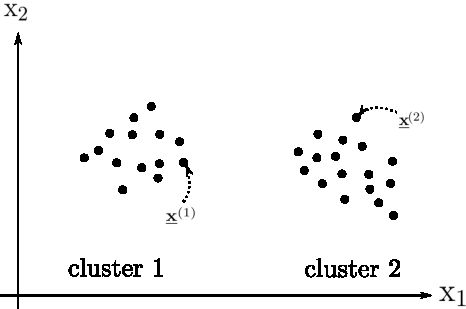
\includegraphics[height=3.5cm]{img/clustering.pdf}
  \caption{Clustering involves discrete-valued arguments.}
  \label{fig:clustering}
\end{figure}
}

\only<2>{

\begin{center}
  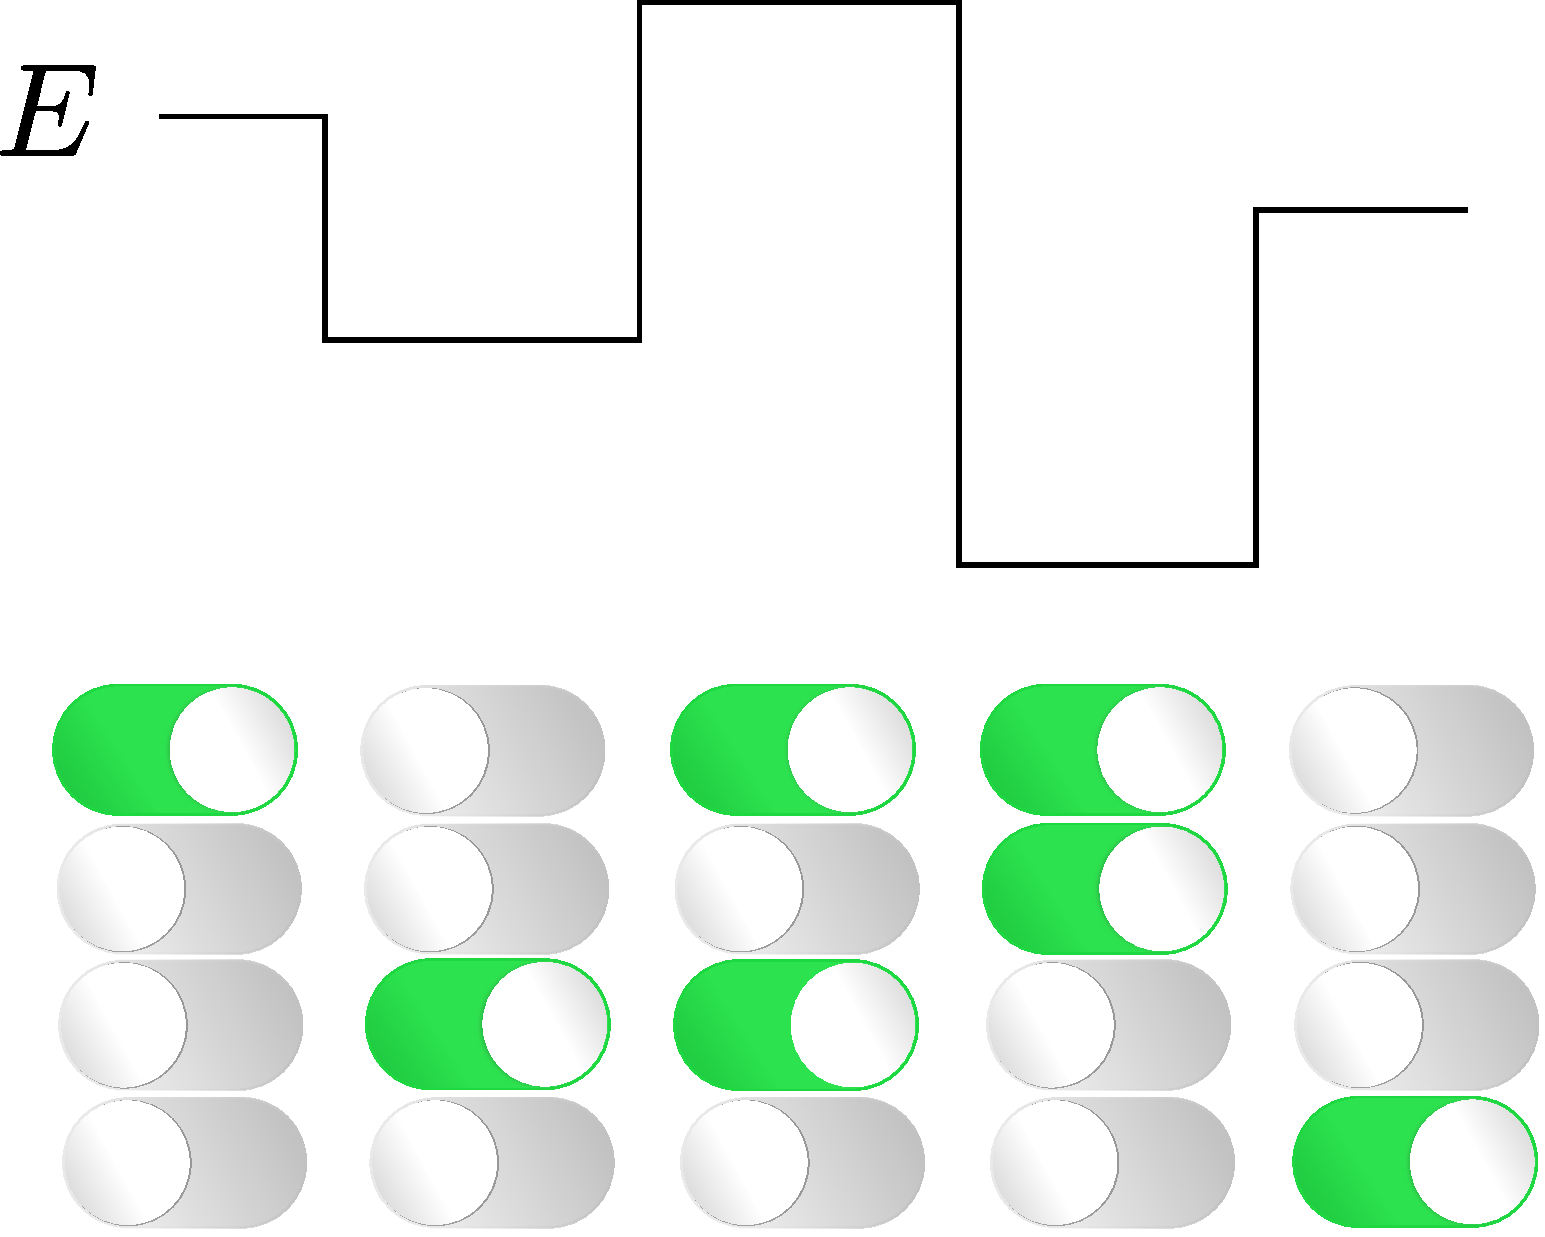
\includegraphics[height=3.5cm]{img/cyberscooty-switch_1-5}
  \notesonly{\captionof{figure}{A combinatorial problem}}
\end{center}
}


\end{frame}

%\newpage

\subsection{Formalization of the discrete optimization problem}

\begin{frame}{\subsecname}

\begin{block}{Setting} 
\begin{itemize}
 \item discrete variables $s_i, \ i = 1, \ldots, N\quad$ (e.g. $s_i \in \{+1, -1\}$  \notesonly{``binary units''} or $s_i \in \mathbb N$) 
 % $s_i \in \{1, 2, \dots 9 \} $ 
 \item \indent short-hand notation: $\vec{s}$ (``state'') -- { $\{\vec{s}\}$ is called state space }
 \item {cost function:} $E: \vec{s} \mapsto E_{(\vec{s})} \in \mathbb{R}$ -- { not restricted to learning problems}
\end{itemize}
\end{block}

We will focus on \textbf{minimization} problems.

\begin{block}{Goal: find state $\vec{s}^*$, such that:} 
\begin{equation*}
	E \eqexcl \min \qquad (\text{desirable global minimum for the cost})
\end{equation*}
Consequently,
\begin{equation*}
	s^* := \argmin E.
\end{equation*}
\end{block}
\end{frame}

\subsubsection{Strategies for discrete optimization}

\begin{frame}{\subsubsecname}

\notesonly{
We want to find the best configuration of a discrete system (e.g.\
state of interacting binary units). Evaluating full search space works only for
very small problems ($\rightarrow 2^N$ possibilities for a problem with $N$
binary units, search space is the set of corners of a
hypercube). A greedy strategy will often get trapped if there are
multiple local minima.
}

\begin{itemize}
\item Evolutionary and genetic algorithms (GA) have been
  motivated by \emph{biological} phenomena of adaptation through
  \emph{mutation} and \emph{selection}.

\vspace{5mm}
  
\item GA and Monte-Carlo-Markov-Chain methods based on a \emph{proposal} and
  \emph{acceptance} strategy ($\rightarrow$ Metropolis) can be interpreted
  as ``learning via trial and error''. \emph{Simulated annealing} falls within MCMC.
\end{itemize}
\end{frame}

